% Adapted from https://raw.githubusercontent.com/MartinThoma/LaTeX-examples/master/tikz/bias-variance/bias-variance.tex

%\usetikzlibrary{arrows.meta,bending}
\tikzset{>=stealth,
    OptimumStyle/.style={align=center,anchor=center,rotate=90,font=\sffamily\scriptsize},
    OverfitStyle/.style={align=center,anchor=west,rotate=0,font=\sffamily\scriptsize},
    UnderfitStyle/.style={align=center,anchor=east,rotate=0,font=\sffamily\scriptsize},
}
%\pgfplotsset{compat=1.17,
%    samples=101,
%    axis lines = left,
%    every axis plot/.append style={line width=2pt},
%}

%\begin{document}
%\fbox{
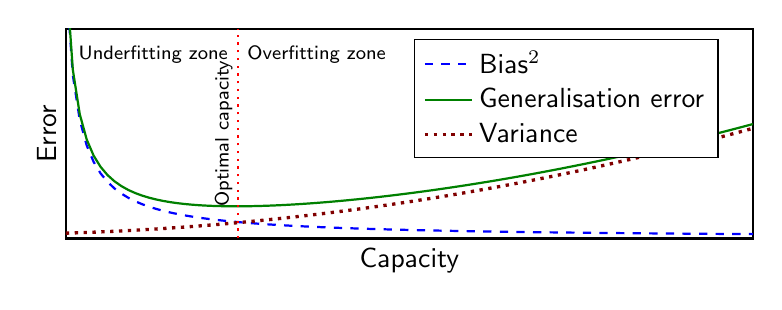
\begin{tikzpicture}[font=\sffamily\sansmath]

    \begin{axis}
        [
        xmin=0,
        xmax=2,
        ymin=0,
        ymax=2,
        xlabel=Capacity,
        ylabel=Error,
        ticks=none,
        xtick={2},
        ytick={2},
        xticklabels={\empty},
        yticklabels={\empty},
        ymajorgrids=true,
        xmajorgrids=true,
        samples=100,
        width=0.85\linewidth,
        height=0.35\linewidth,
        axis line style = thick,
        legend cell align={left},
        legend style={at={(0.95,0.95)},anchor=north east}
        ]
        \addplot[domain=0.00:2.0, blue, dashed, thick] {0.25/(3*x+0.1)};   % Error due to bias
        \addlegendentry{Bias$^2$}
        \addplot[domain=0.00:2.0, green!50!black, thick] {0.25/(3*x+0.1) + 0.1*x + 0.2 *x*x + 0.05};  % Generalisation error
        \addlegendentry{Generalisation error}
        \addplot[domain=0.00:2.0, red!50!black, dotted, very thick] {0.1*x + 0.2 *x*x + 0.05};  % Error due to variance
        \addlegendentry{Variance}
%      \addplot[domain=0.39:1.61,black] {3*(x-2)*x+3.8};  %Total error
        \addplot[dotted, red, thick] coordinates {(0.5,0) (0.5,2)};           %Optimum model complexity
%        \addplot[thin, <->] coordinates {(1.5,0.1) (1.5,0.65)};       %Optimum model complexity

        \node[OptimumStyle] at (axis cs:0.46,1.0) {Optimal capacity};
        \node[UnderfitStyle] at (axis cs:0.5,1.75) {Underfitting zone};
        \node[OverfitStyle] at (axis cs:0.5,1.75) {Overfitting zone};
%        \node[OverfitStyle] at (axis cs:1.5,0.33) {Generalisation gap};
%      \node[anchor=south west,text=Maroon] at (axis cs:1.4,0.4){Bias\textsuperscript{2}};
%      \node[anchor=north west,text=TealBlue] at (axis cs:1.4,0.85){Variance};
%      \node[anchor=south east,align=center] at (axis cs:1.5,1.5){Total\\error};
%        \legend{}
    \end{axis}
\end{tikzpicture}
%}

%\end{document}